\documentclass[conference]{IEEEtran}
\usepackage{graphicx}
\usepackage{booktabs}
\usepackage{amsmath}
\usepackage{url}
\usepackage[hidelinks]{hyperref}

\begin{document}

\title{Testing ML Link Adaptation Under RF Impairments:\\
Failure Detection, Diagnosis and Safe Fallback}

\author{\IEEEauthorblockN{Arnav [Surname]}
\IEEEauthorblockA{{[Department, University]}\\
Email: [your email] \quad Code: [GitHub link]}}

\maketitle

\begin{abstract}
Machine-learning (ML) features are entering the 5G/6G air interface, but a model that
improves throughput on the channels it was trained on can fail silently elsewhere. For test
and measurement, the open question is less ``is the ML better?'' than ``where can it be
trusted, and how is failure detected?''. We build a simulation framework in the spirit of a
software call box: an NR-like PDSCH link with TS~38.101-4 fading profiles and four switchable
RF impairments (PA compression, IQ imbalance, phase noise, residual CFO), a BLER-table
abstraction for fast closed-loop runs, an outer-loop link adaptation (OLLA) baseline, and an
ML link-adaptation model as the device under test. Across 52 channel/impairment scenarios,
the ML model beats a tuned OLLA by +2 to +15\% on clean fading channels, including one it never
saw, but loses up to 89\% at high SNR under moderate or severe impairments. A self-check
that compares the model's predicted ACK probability with observed ACKs detects these failures
far better than input-distribution monitoring (AUROC 0.89 vs.\ 0.68). A four-view CNN names
the impairment correctly in all 23 high-SNR failure cases, and a fallback to OLLA reduces the
average loss in failure cases from $-35.8\%$ to $-6.9\%$ while keeping most of the gain
elsewhere ($+9.0\%$ to $+8.1\%$). One failure remains invisible to the self-check: an
over-cautious model on a non-fading channel.
\end{abstract}

\section{Introduction}
Link adaptation (LA) selects a modulation and coding scheme (MCS) for every slot from
imperfect channel-state reports. The standard approach, OLLA~\cite{nakamura2002}, adds an
offset to the reported SNR that moves up on ACK and down on NACK, holding the block error rate
(BLER) near a target of 10\%. ML-based LA can exploit structure OLLA ignores, but it raises a
verification problem that is central to AI/ML in the NR air interface~\cite{tr38843}: a model
can perform well in its training conditions and degrade outside them without any visible
sign.

This work treats that as a test problem and builds a miniature version of the workflow a
call-box team would need: \emph{feature} (an ML LA model), \emph{test} (sweeps over
conformance channels and RF impairments), \emph{diagnose} (detect and name the cause of
failure), and \emph{mitigate} (fall back safely). Our contributions are:
\begin{itemize}
\item an open simulation framework with a full NR-like PHY, conformance fading profiles,
four calibrated impairment models, and a fast BLER-table closed loop (Sec.~\ref{sec:sys});
\item a map of where an ML LA model wins and fails across 52 scenarios (Sec.~\ref{sec:e2});
\item a comparison of two failure detectors using only gNB-side information, showing that a
prediction self-check outperforms input out-of-distribution (OOD) detection
(Sec.~\ref{sec:e3});
\item an impairment classifier on instrument-style views, and a diagnosis-aware fallback that
removes most of the downside of the ML model (Secs.~\ref{sec:e4},~\ref{sec:e5}).
\end{itemize}

\section{System Model}\label{sec:sys}

\subsection{Link-level chain}
We simulate a single-layer downlink with Sionna~\cite{sionna} (PyTorch backend): 30~kHz
subcarrier spacing, 24 PRBs, FFT size 512 ($f_s=15.36$~MHz), normal cyclic prefix, 14-symbol
slots, and type-1 comb DMRS on symbols 2 and 11 with no data on DMRS symbols, leaving 3456
data resource elements per slot. MCS and transport-block size follow TS~38.214
Table~5.1.3.1-1~\cite{ts38214}; MCS 0--2 are excluded because the LDPC encoder used does not
support rates below 1/5. The receiver uses least-squares channel estimation with linear
interpolation in frequency and time, MRC, soft demapping, and 20-iteration belief-propagation
LDPC decoding.

Channels are the TS~38.101-4~\cite{ts38101_4} conformance profiles TDLA30-10, TDLB100-400 and
TDLC300-100 (TR~38.901 TDL models~\cite{tr38901}) plus AWGN. The channel is held constant
within each OFDM symbol, which captures channel ageing between DMRS symbols but ignores
Doppler-induced ICI (below 1.5\% of the subcarrier spacing here).

\subsection{RF impairments}
Impairments are placed where they occur in a downlink test: PA compression at the transmitter
(call-box side), and residual CFO, phase noise and IQ imbalance at the UE receiver, applied
after thermal noise. The PA follows the Rapp model~\cite{rapp1991} with smoothness $p=2$ and
input back-off as the severity parameter. IQ imbalance is $y=\mu x+\nu x^*$ with gain and phase
mismatch; phase noise is a Wiener process with a given 3-dB linewidth; CFO is a constant
rotation normalised to the subcarrier spacing. Each has mild, moderate and severe settings
calibrated to cap post-equalisation SINR at roughly 27--30, 18--21 and 12--16~dB (AWGN, 45~dB
SNR). With the clean case this gives 13 settings, and with the four channels, 52 scenarios.

\subsection{BLER tables and closed loop}
Decoding is too slow for long closed-loop runs, so each scenario is simulated once (on a GPU)
and summarised per MCS by a three-parameter fit against the \emph{slot SNR}, the wideband SNR
of that slot's fading realisation:
\begin{equation}
\mathrm{BLER}(s)=1-(1-f)\,\sigma\!\big(k(s-s_{50})\big),
\end{equation}
with centre $s_{50}$, steepness $k$ and error floor $f$, fitted by maximum likelihood to
per-block outcomes. The slot SNR excludes impairments: the scheduler cannot see them, so they
appear only as shifted curves or error floors. Conditioning on wideband SNR treats in-slot
frequency selectivity as randomness inside each curve rather than mapping it exactly, as
EESM/MIESM abstractions would.

The closed loop runs one iteration per 0.5~ms slot. The true slot SNR follows a TDL fading
process sampled at the slot rate. The scheduler sees an SNR report every 5~ms, measured 2~ms
earlier, with 1~dB error and 1~dB quantisation, plus noisy Doppler and delay-spread
estimates, and receives ACK/NACK after 1~ms. ACKs are drawn from the BLER table at the true
slot SNR of the true scenario. There are no HARQ retransmissions, and a single full-buffer user
is assumed.

\section{Link Adaptation Under Test}

\subsection{Baseline: OLLA}
The inner loop picks the highest MCS whose AWGN-curve SNR for 10\% BLER is below the report
plus offset; the offset decreases by $\Delta_{\downarrow}$ on NACK and increases by
$\Delta_{\uparrow}=\Delta_{\downarrow}\,t/(1-t)$ on ACK, so the BLER converges to $t=0.1$. A
sweep of $\Delta_{\downarrow}\in[0.1,2]$~dB showed throughput within 1--4\% across step
sizes; we use 0.5~dB. OLLA holds 10.0\% BLER in all four clean channels.

\subsection{Device under test: ML link adaptation}
The model sees ten gNB-side features: the latest report, its trend and age, log Doppler and
delay-spread estimates, ACK rates over the last 8 and 32 feedbacks, a background OLLA-style
offset, the last MCS, and the current NACK streak. An MLP (two hidden layers of 128 units)
outputs, for every MCS at once, the probability that a block sent with that MCS will be ACKed.
Because the BLER tables give a label for every MCS in every slot, training needs no
exploration: targets are $1-\mathrm{BLER}_m$ at the true slot SNR, with binary cross-entropy
loss. The MCS is then chosen either to maximise TBS$\times P(\mathrm{ACK})$ or, in the mode we
evaluate unless stated, as the highest MCS with $P(\mathrm{ACK})\ge0.9$ (same target as OLLA).

Training data come from two rounds: closed-loop runs with an exploring OLLA, then runs with
the round-0 model itself (DAgger~\cite{dagger}), so the model also sees the ACK patterns its own
decisions produce. Training is deliberately limited to TDLA30-10 and TDLB100-400 without
impairments, at average SNRs drawn from 0--28~dB. Everything else is out of distribution.

\section{Experiments and Results}

\subsection{E1: ML vs.\ OLLA on clean channels}\label{sec:e1}
Fig.~\ref{fig:e1} compares the ML model with OLLA and with an oracle that knows the true slot
SNR (3 seeds, 5~s of traffic each). In the training channels, the ML model gains +2 to +9\%
(TDLA30-10) and +7 to +13\% (TDLB100-400) at about the same BLER. It generalises to the unseen
TDLC300-100 (+9 to +15\%), but on the unseen AWGN channel it loses 21\% at 5--10~dB: its
inputs (no Doppler, no delay spread) lie outside the training range and it becomes
over-cautious (0\% BLER). One mechanism behind the gain is visible in the tables: under fading,
MCS~16 needs more SNR than MCS~17 while carrying less data. OLLA's AWGN-based mapping still
uses MCS~16 (about 12\% of slots at 13~dB in TDLA30-10); the ML model never does.

\begin{figure*}[t]
\centering
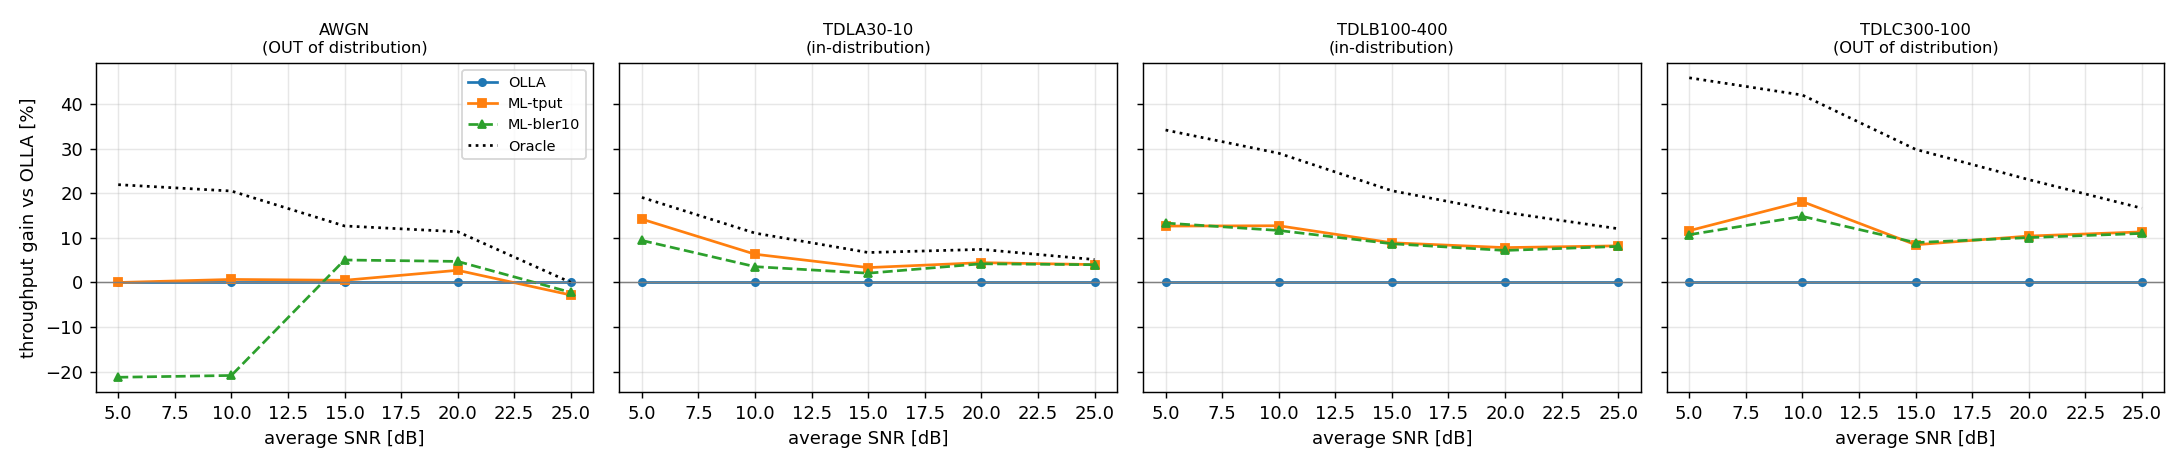
\includegraphics[width=\textwidth]{e1_compare.png}
\caption{E1: throughput gain over OLLA on clean channels. TDLA30-10 and TDLB100-400 are
training conditions; AWGN and TDLC300-100 were never seen. The oracle knows the true slot
SNR and is an upper bound.}
\label{fig:e1}
\end{figure*}

\begin{figure*}[t]
\centering
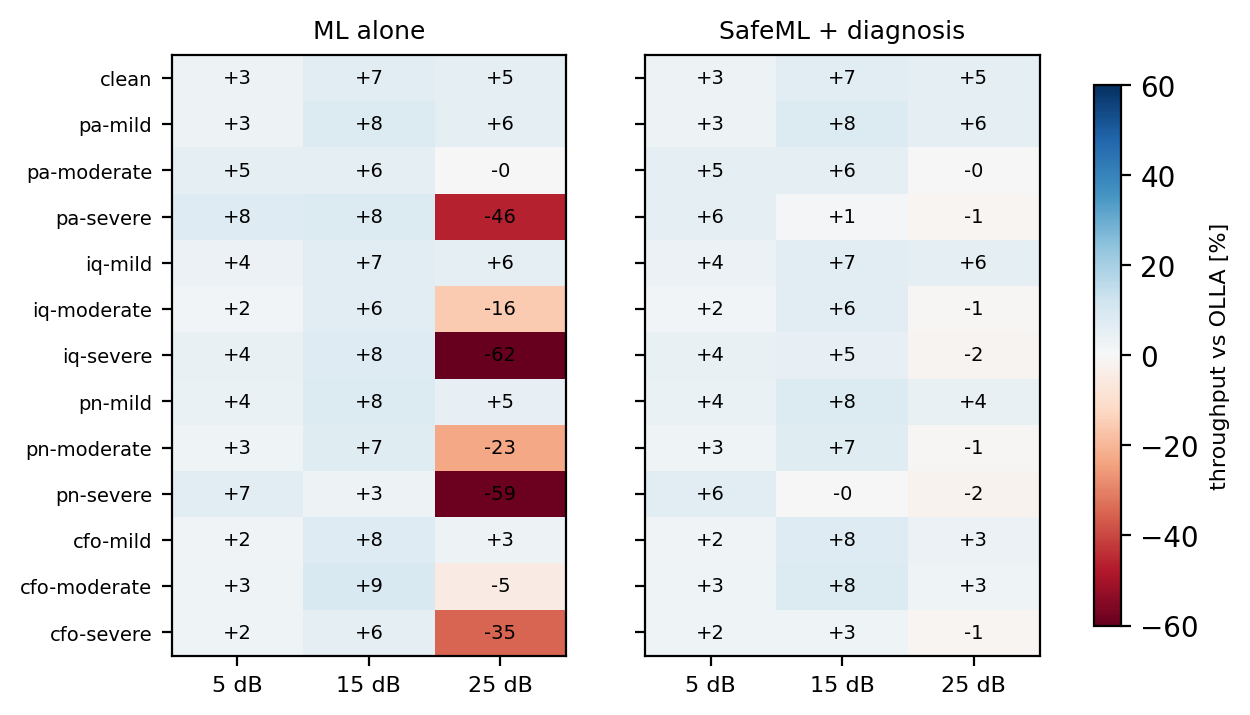
\includegraphics[width=0.78\textwidth]{fig_e2_compact.png}
\caption{E2/E5: throughput vs.\ OLLA per impairment setting and SNR, averaged over the four
channels. Left: ML alone. Right: ML with the self-check, fallback and diagnosis.}
\label{fig:e2}
\end{figure*}

\begin{figure*}[t]
\centering
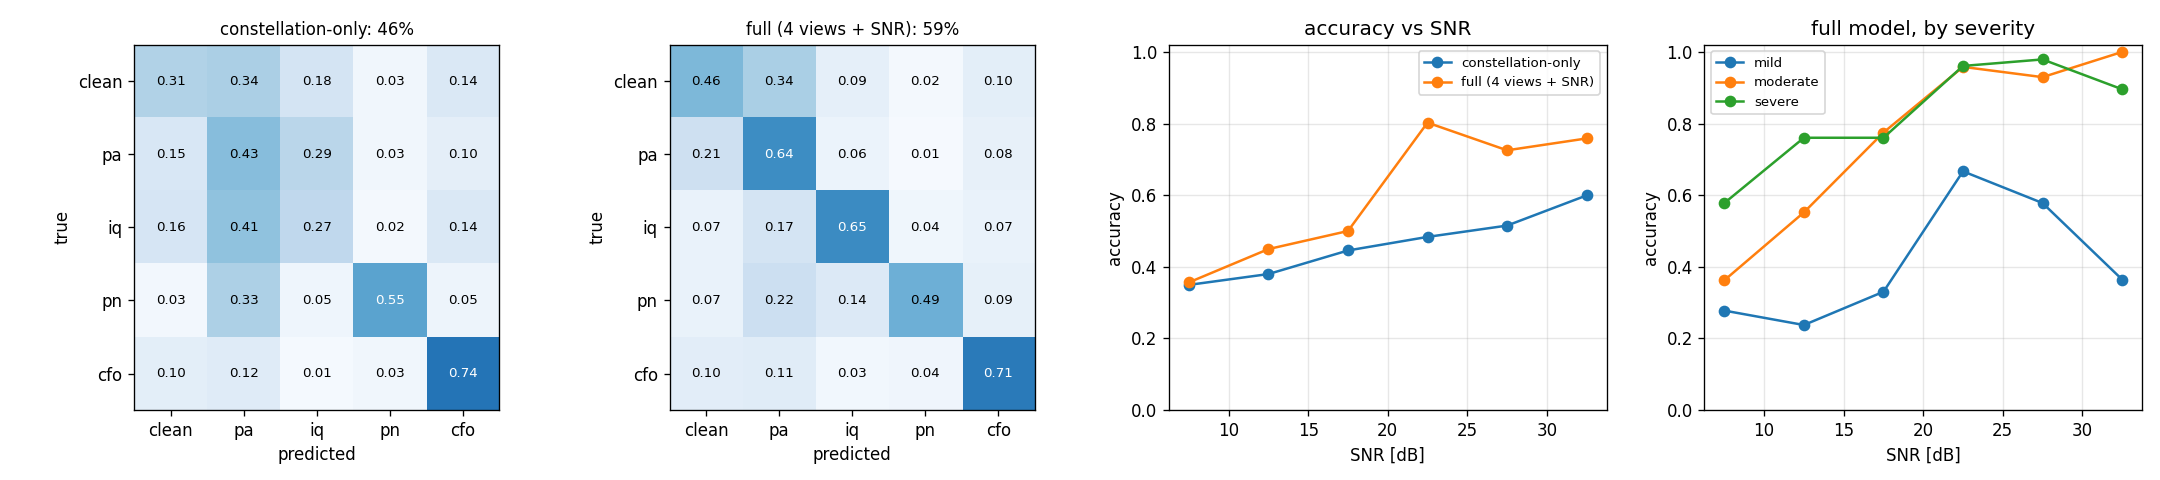
\includegraphics[width=\textwidth]{e4_diagnosis.png}
\caption{E4: confusion matrices (constellation-only vs.\ four views + SNR), accuracy vs.\
SNR, and accuracy by severity.}
\label{fig:e4}
\end{figure*}

\subsection{E2: where the ML model fails}\label{sec:e2}
We ran the ML model and OLLA on identical fading and noise (common random numbers) for all 52
scenarios at 5, 15 and 25~dB (2 seeds, 3~s each). The ML model is more than 5\% worse than
OLLA in 34 of 156 cells, with a worst case of $-89\%$. Fig.~\ref{fig:e2} (left) shows the
pattern: failures concentrate at 25~dB with moderate or severe impairments. There, the reports
promise a high SNR, but the impairment caps the achievable SINR below what the chosen MCS
needs. At 5~dB the same impairments are buried under thermal noise and the model still gains
about 2--8\%. OLLA is robust by construction, since its ACK-driven offset absorbs any constant
SNR penalty the reports hide.



\subsection{E3: detecting failure}\label{sec:e3}
Both detectors use only information a gNB or call box has. \emph{Input OOD} scores how far the
feature vector is from the training data (Mahalanobis distance~\cite{lee2018}, averaged over
250~ms). The \emph{self-check} compares the model's mean predicted $P(\mathrm{ACK})$ for its
chosen MCS with the observed ACK rate in the same window. Thresholds are the 99th percentile
over training-condition windows on separate seeds. A window is labelled a failure if ML
delivers more than 5\% less data than OLLA in it.

\begin{table}[t]
\centering
\caption{E3: detectors over 3744 windows of 250~ms (22.8\% failures)}
\label{tab:e3}
\begin{tabular}{lccc}
\toprule
Detector & AUROC & Caught & False alarms \\
\midrule
Input OOD (Mahalanobis) & 0.68 & 66\% & 39\% \\
Prediction self-check   & 0.89 & 66\% & 20\% \\
\bottomrule
\end{tabular}
\par\vspace{2pt}\footnotesize False alarms: share of non-failure windows flagged (0\% in training conditions for both).
\end{table}

Table~\ref{tab:e3} shows the self-check is clearly better. Input OOD flags TDLC300-100, whose
long delay spread is unusual but where the model does well, and misses impairments that leave
the inputs unchanged. ``The inputs look unusual'' is a weak proxy for ``the model is wrong.''
Neither detector sees the AWGN failure: at 5~dB the model predicts 97\% ACK for MCS~5 and
observes 100\%, so its own choices look fine. The loss lies in the higher MCS it never tries,
and detecting it requires probing, which OLLA does by design.

\subsection{E4: naming the impairment}\label{sec:e4}
A small CNN classifies one slot of equalised symbols into clean, PA, IQ, phase noise or CFO.
Instead of the constellation alone, it receives four instrument-style 32$\times$32 views
(Fig.~\ref{fig:views}): the constellation; radial error vs.\ amplitude; \emph{image leakage},
the error on subcarrier $k$ multiplied by the decided symbol on $-k$, which IQ imbalance
shifts off-centre; and phase error vs.\ OFDM symbol, where CFO drifts and phase noise
wanders. Reference symbols are hard decisions, so no genie data is used. The CNN also gets
the SNR, which a call box knows because it sets the noise level.

\begin{figure}[t]
\centering
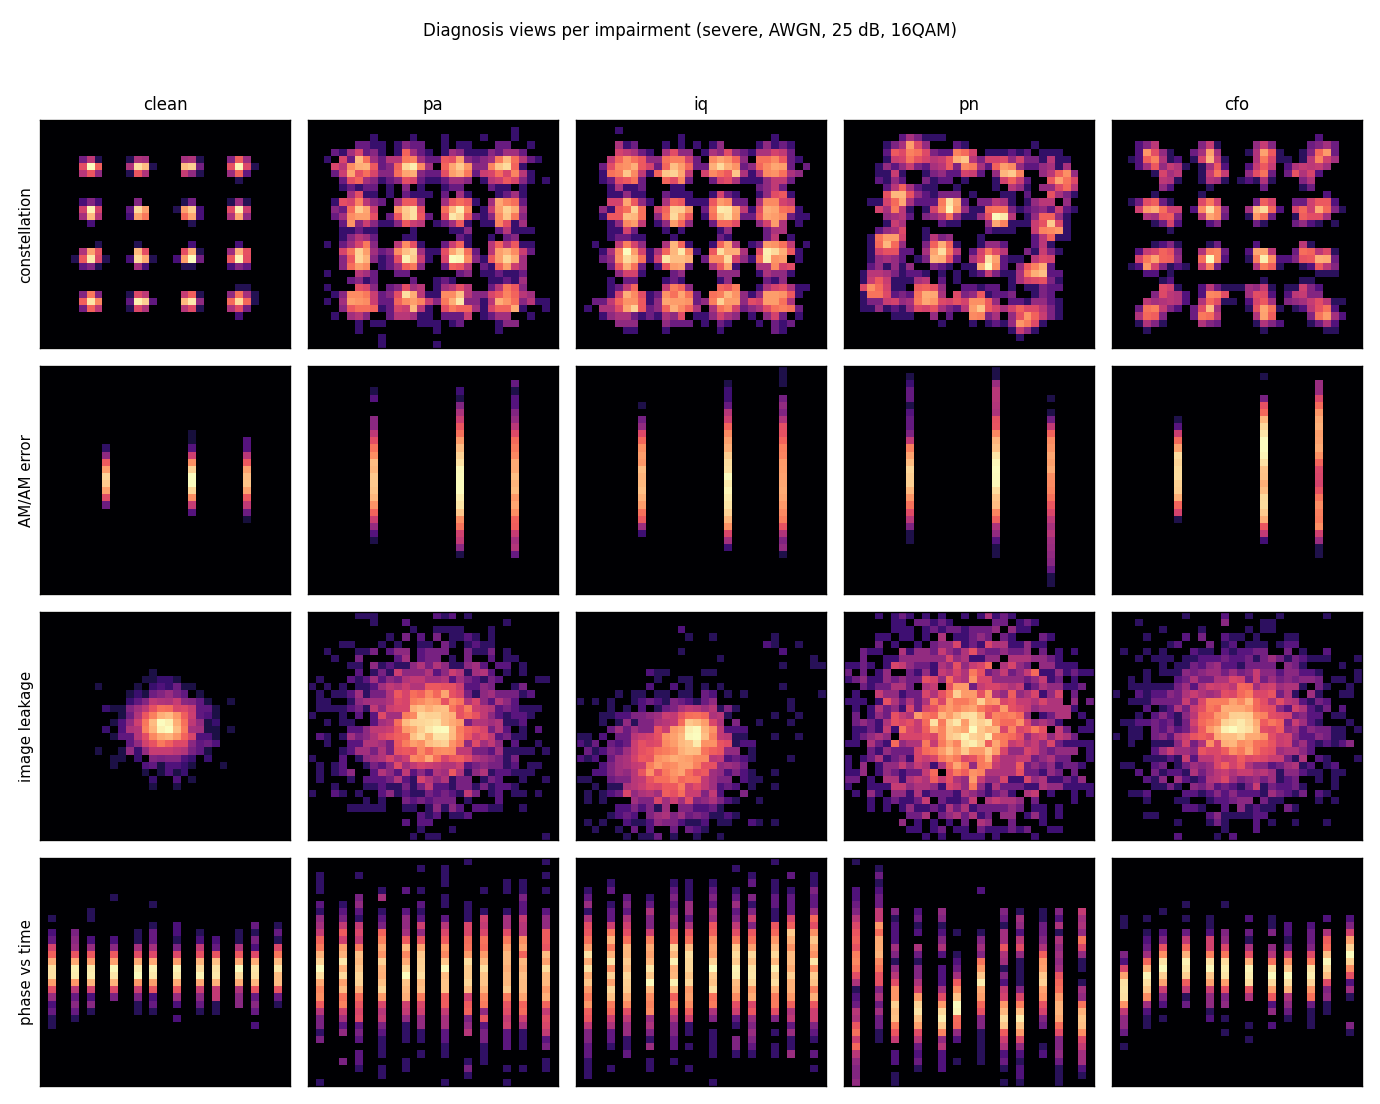
\includegraphics[width=\columnwidth]{diagnosis_views.png}
\caption{Diagnosis views for each class (severe level, AWGN, 25~dB, 16QAM).}
\label{fig:views}
\end{figure}

Trained on 8000 slots across all channels, SNRs of 5--35~dB and all severities, and tested on
2400 unseen slots, the constellation-only CNN reaches 46\% and the full model 59\% (5 classes,
Fig.~\ref{fig:e4}). For moderate and severe impairments at SNR $\ge 20$~dB, accuracy is about
95\%. The image-leakage view cuts IQ-to-PA confusion from 0.41 to 0.17. PA compression does
not appear as an inward pull of the outer points: in OFDM the clipping distortion spreads
over all subcarriers and behaves like additive noise (Bussgang~\cite{bussgang1952}), so it is
only recognisable as more noise than the SNR explains. Mild impairments, and any impairment
at low SNR, are mostly undiagnosable because their distortion is below thermal noise.


\subsection{E5: safe fallback}\label{sec:e5}
SafeML runs the ML model while keeping OLLA warm on the same ACKs. Over the last 200 resolved
slots it compares predicted and observed ACK rates; if the model is over-confident by more
than 0.16, control passes to OLLA. With diagnosis enabled, an impairment verdict keeps OLLA in
control (hardware faults persist), while ``clean'' lets ML retry after 1~s. Diagnosis is only
trusted at SNR $\ge 15$~dB, following E4. A first version with a 0.08 margin was triggered by
ordinary slow fades and kept only $+2.4\%$ of the ML gain; real failures show gaps of
0.3--0.8, so the wider margin loses nothing in detection.

\begin{table}[t]
\centering
\caption{E5: throughput vs.\ OLLA over 156 scenario/SNR cells}
\label{tab:e5}
\begin{tabular}{lccc}
\toprule
Policy & ML-fail cells & ML-win cells & Worst \\
\midrule
ML alone          & $-35.8\%$ & $+9.0\%$ & $-89\%$ \\
SafeML            & $-9.1\%$  & $+8.2\%$ & $-21\%$ \\
SafeML + diagnosis & $-6.9\%$ & $+8.1\%$ & $-21\%$ \\
\bottomrule
\end{tabular}
\par\vspace{2pt}\footnotesize 34 cells where ML alone is $>5\%$ below OLLA; 102 where it is $>2\%$ above.
\end{table}

Table~\ref{tab:e5} and Fig.~\ref{fig:e5} show the result: the fallback removes almost all of
the downside and keeps almost all of the upside. The diagnosis named the correct impairment in
all 23 high-SNR failure cells. The remaining worst case ($-21\%$) is AWGN at 5~dB, the
over-caution failure no self-check can see.

\begin{figure}[!t]
\centering
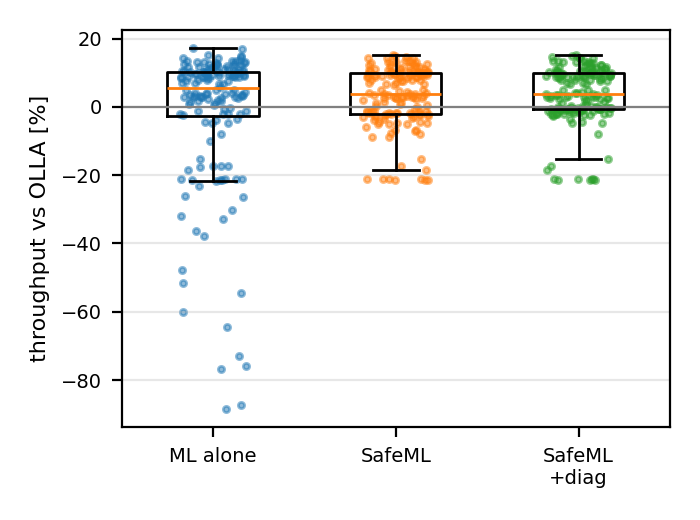
\includegraphics[width=0.92\columnwidth]{fig_e5_summary.png}
\caption{E5: throughput vs.\ OLLA in each of the 156 cells, per policy.}
\label{fig:e5}
\end{figure}

\section{Limitations}
All results are simulation. The impairment models are simplified and not calibrated to
specific hardware. The BLER abstraction conditions on wideband SNR and omits HARQ combining.
There is no PTRS, so phase noise is uncorrected between DMRS symbols, which is pessimistic for
FR1. The diagnosis assumes one impairment at a time. The stress test uses 2 seeds per cell;
E1 uses 3. The harness exposes a mock instrument interface so a real call box could replace
the simulator, but this has not been tested.

\section{Conclusion}
An ML link-adaptation model can beat a tuned OLLA by up to 15\% and still fail by up to 89\%
under impairments its inputs cannot reveal. For testing such features, three findings stand
out: (i) failure regions are structured (high SNR, significant impairment) and can be mapped
by sweeping conformance channels against impairment severity; (ii) a self-check of the model's
own predictions detects failure far better than input-distribution monitoring, but cannot
see over-caution; (iii) instrument-style views plus the known SNR make the cause of failure
identifiable, enabling a fallback that keeps the ML gain where it is real. Natural next steps
are combined impairments, HARQ-aware abstraction, probing to expose over-caution, and
validation against measured impairment data.

\begin{thebibliography}{10}
\bibitem{nakamura2002} M.~Nakamura, Y.~Awad, and S.~Vadgama, ``Adaptive control of link
adaptation for high speed downlink packet access (HSDPA) in W-CDMA,'' in \emph{Proc. WPMC},
2002.
\bibitem{tr38843} 3GPP, ``Study on artificial intelligence (AI)/machine learning (ML) for NR
air interface,'' TR~38.843.
\bibitem{sionna} J.~Hoydis \emph{et al.}, ``Sionna: An open-source library for next-generation
physical layer research,'' arXiv:2203.11854, 2022.
\bibitem{ts38214} 3GPP, ``NR; Physical layer procedures for data,'' TS~38.214.
\bibitem{ts38101_4} 3GPP, ``NR; User Equipment (UE) radio transmission and reception; Part 4:
Performance requirements,'' TS~38.101-4.
\bibitem{tr38901} 3GPP, ``Study on channel model for frequencies from 0.5 to 100 GHz,''
TR~38.901.
\bibitem{rapp1991} C.~Rapp, ``Effects of HPA-nonlinearity on a 4-DPSK/OFDM-signal for a
digital sound broadcasting system,'' in \emph{Proc. 2nd European Conf. Satellite
Communications}, 1991.
\bibitem{dagger} S.~Ross, G.~Gordon, and D.~Bagnell, ``A reduction of imitation learning and
structured prediction to no-regret online learning,'' in \emph{Proc. AISTATS}, 2011.
\bibitem{lee2018} K.~Lee, K.~Lee, H.~Lee, and J.~Shin, ``A simple unified framework for
detecting out-of-distribution samples and adversarial attacks,'' in \emph{Proc. NeurIPS},
2018.
\bibitem{bussgang1952} J.~J.~Bussgang, ``Crosscorrelation functions of amplitude-distorted
Gaussian signals,'' MIT Research Laboratory of Electronics, Tech. Rep. 216, 1952.
\end{thebibliography}

\end{document}
